\chapter{ Ambiente di Lavoro}

Per far funzionare \LaTeX{} sul vostro computer dovete scaricare anche un
compilatore, che potete trovare a questo all'indirizzo
\url{https://miktex.org/download}. L'installazione è facile ma il completamento
potrebbe richiedere un po' di tempo. Siate pazienti.
Per gli scopi di questo corso utilizzeremo \textbf{TeXnicCenter}, un comodo IDE
che potete scaricare gratuitamente all'indirizzo
\url{http://www.texniccenter.org/download/}.
Ovviamente avrete bisogno anche di un visualizzatore PDF, in questo caso noi
consigliamo un lettore PDF leggero e veloce (cosa che Adobe Reader non è), che
ci sarà molto utile in quanto dovremo aprirlo ripetutamente: il lettore PDF in
questione si chiama SumatraPDF ed è gratuitamente scaricabile al seguente
indirizzo \url{https://www.sumatrapdfreader.org/download-free-pdf-viewer.html}.
In ogni caso siete liberi di utilizzare il lettore PDF che più preferite.

\section{Windows e TeXnicCenter}

Durante la prefazione (che nessuno di voi avrà certamente letto) abbiamo
parlato di IDE. Per il nostro corso ne utilizzeremo uno (come già detto sopra)
e in questo capitolo vedremo un attimo le sue funzionalità, giusto per prendere
mano con l'ambiente che dovremo usare.

Se avete installato TeXnicCenter sul vostro computer per la prima volta e lo
state aprendo solo ora vi chiederà alcune informazioni riguardo al lettore DVI
e PDF da usare. Riguardo al lettore DVI potete pure lasciare i campi vuoti,
mentre per il lettore PDF premete i tre puntini accando alla prima casella di
testo, e selezionate nel vostro hard disk l'eseguibile del lettore PDF che più
preferite.

Prima di tutto, alla apertura del programma ci troveremo ad una schermata
vuota, in cui possiamo vedere diversi bottoni.

\begin{figure}[H]
  \centering
  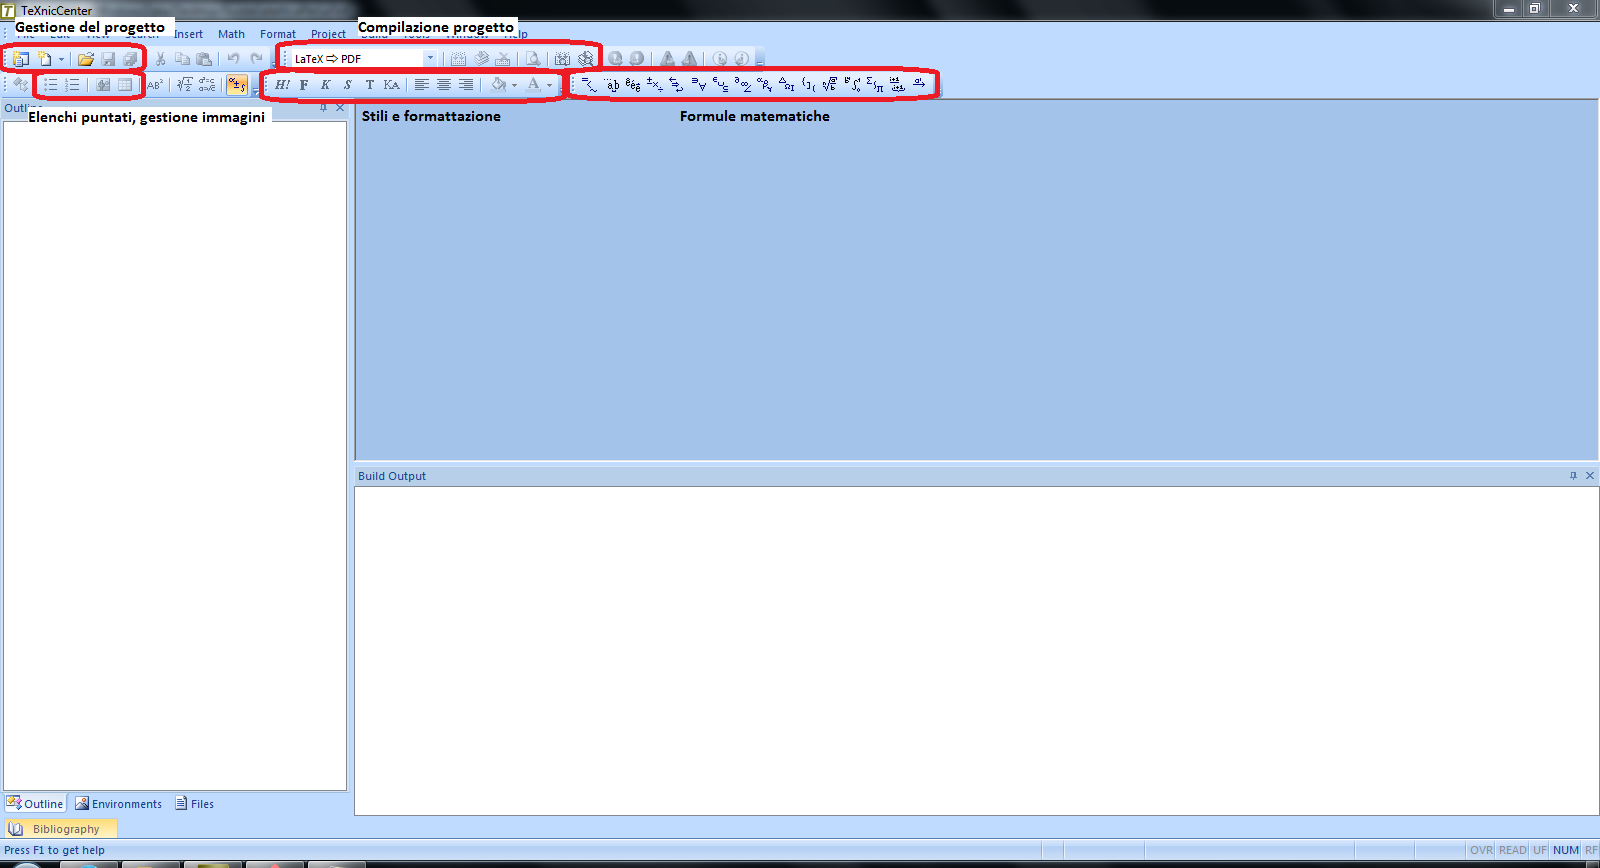
\includegraphics[scale=0.35]{texniccenterprincipale}
  \caption{Schermata principale di TeXnicCenter}
\end{figure}

Come possiamo vedere dall'immagine\footnote{Sappiamo che si vede poco
ma questo è il meglio che siamo riusciti a fare} notiamo partendo da in alto
a sinistra e scorrendo verso destra che inizialmente troviamo dei bottoni per
gestire il progetto (o per crearne di nuovi).
Abbiamo subito dopo le opzioni per la compilazione: il menù a tendina ci
permette di selezionare che tipo di output vogliamo (se PDF o altri formati) e
i bottoni accanto a questo menù ci permettono di lanciare la compilazione
del progetto.
Nella seconda riga troviamo le impostazioni per aggiungere elenchi puntati e
numerati, seguiti dai bottoni per aggiungere immagini e tabelle. Nel penultimo
riquadro ci sono i classici bottoni per impostare gli stili di formattazione
(quelli che siamo abituati ad avere in Word per intenderci).
Alla fine troviamo i bottoni per l'inserimento di formule matematiche, che
tratteremo più avanti in questa guida.

\subsection{Creare un progetto}

Iniziamo ora la creazione di un progetto.
Clicchiamo su \texttt{New Project} e selezioniamo l'unico modello diponibile,
ovvero quello vuoto. Spuntiamo la casellina \texttt{Uses BibTeX} nella sezione
\texttt{Features}, e diamo un nome al nostro progetto. Fatto ciò il bottone
\texttt{Ok} dovrebbe essersi sbloccato, e lo clicchiamo. Il programma creerà
le basi necessarie per cominciare un nuovo progetto!\footnote{Nota, se volete
potete selezionarvi il percorso dove salvare il progetto che preferite.}
Il progetto che avremo davanti è però vuoto, e consisterà di un unico file: per
progetti \LaTeX{} grandi è generalmente buona pratica separare quelle che sono
le impostazioni del progetto (come configurazione dei pacchetti e importazione
degli stessi) dal contenuto (ovvero quello che è il vero e proprio documento).
Questo permette poi di eseguire modifiche più facilmente, e di avere un maggior
ordine nel progetto stesso.
La struttura consigliata potrebbe essere:
\begin{verbatim}
 main.tex
 ...
 res/
 -- config/
 ---- config.tex
 ---- package.tex
 -- sections/
 -- img/
 listOfSections.tex
\end{verbatim}

Spiegheremo brevemente perché:
\begin{itemize}
  \item Il \texttt{main.tex} è buona pratica che contenga solo il codice
necessario per importare i vari pezzi del progetto, e per darne le informazioni
di base
  \item In \texttt{res/} ci saranno le risorse vere e proprie del progetto, che
sono composte dai file di configurazione, dalle varie immagini e da altri file
TeX, che possono rappresentare capitoli o parti (la suddivisione è a proprio
piacimento)
  \begin{itemize}
   \item In \texttt{config/} abbiamo il file dove configurare i vari pacchetti
(per esempio scriviamo li se preferiamo avere i link di colore rosso al posto
di blu), mentre nell'altro file, \texttt{package.tex} abbiamo tutte le
importazioni necessarie per far compilare il documento. In questa maniera, se
un pacchetto dovesse a detta del compilatore risultare mancante potremmo subito
controllare se avrà ragione o meno\footnote{E l'avrà perché i computer sono
macchine, e le macchine se programmate bene hanno la tendenza e non sbagliare.}
  \item In \texttt{img} metteremo tutte le immagini, così da avere un unico
posto dove salvarle e eviteremo in questa maniera di spargerle su tutto il
progetto.
  \item \texttt{listOfSections} grazie alla \textit{keyword} \verb!\include!
possiamo includere diversi file, ed è consigliato includerli qui % TODO finish
  \end{itemize}

\end{itemize}

